\section{Preventivo}
Sigle identificative per i ruoli indicati nelle tabelle e nei grafici:
\begin{itemize}
    \item \textbf{RE}: Responsabile;
    \item \textbf{AM}: Amministratore;
    \item \textbf{AN}: Analista;
    \item \textbf{PT}: Progettista;
    \item \textbf{PR}: Programmatore;
    \item \textbf{VE}: Verificatore.
\end{itemize}

{	
\rowcolors{2}{grigetto}{white}
\renewcommand{\arraystretch}{2}
\centering
\begin{longtable}[h!]{ C{3cm} C{4cm}}
\caption{Tabella con i costi per ogni ruolo}\\
\rowcolor{darkblue}

\textcolor{white}{\textbf{Ruolo}} & \textcolor{white}{\textbf{Costo per ora (in \euro{})}}\\

Responsabile   & 30 \\
Amministratore & 20 \\
Analista       & 25 \\
Progettista    & 22 \\
Programmatore  & 15 \\
Verificatore   & 15 \\
\end{longtable}
}

\clearpage
\subsection{Fase di Analisi}

\subsubsection{Divisione Oraria}
La seguente tabella rappresenta la distribuzione oraria dei ruoli per ogni componente del gruppo:
{
\rowcolors{2}{grigetto}{white}
\renewcommand{\arraystretch}{2}
\begin{longtable}[h!] { C{4cm} C{1cm} C{1cm} C{1cm} C{1cm} C{1cm} C{1cm} C{3cm}}
\caption{Tabella della divisione oraria di Analisi}	\\
\rowcolor{darkblue}

\textcolor{white}{\textbf{Membro del gruppo}} & 
\textcolor{white}{\textbf{RE}} & 
\textcolor{white}{\textbf{AM}} & 
\textcolor{white}{\textbf{AN}} & 
\textcolor{white}{\textbf{PT}} & 
\textcolor{white}{\textbf{PR}} & 
\textcolor{white}{\textbf{VE}} & 
\textcolor{white}{\textbf{Ore complessive}}\\	
\endhead

\MC{}                     &  0 &  7 &  12 & 0 & 0 & 11 &  30 \\
\LD{}                     &  0 &  5 &  16 & 0 & 0 &  9 &  30 \\
\CE{}                     &  0 &  0 &  21 & 0 & 0 &  9 &  30 \\
\SE{}                     & 15 &  2 &   8 & 0 & 0 &  5 &  30 \\
\PF{}                     &  0 &  0 &  21 & 0 & 0 &  9 &  30 \\
\DF{}                     &  0 &  7 &  16 & 0 & 0 &  7 &  30 \\
\BR{}                     &  0 &  5 &  11 & 0 & 0 & 14 &  30 \\
\AT{}                     &  4 & 12 &   9 & 0 & 0 &  5 &  30 \\
\textbf{Ore totali ruolo} & 19 & 38 & 114 & 0 & 0 & 69 & 240 \\

\end{longtable}
}

La suddivisione delle ore svolte da ciascun componente del gruppo per ogni ruolo viene rappresentata nel seguente istogramma:
\begin{figure}[h!]
	\centering	
	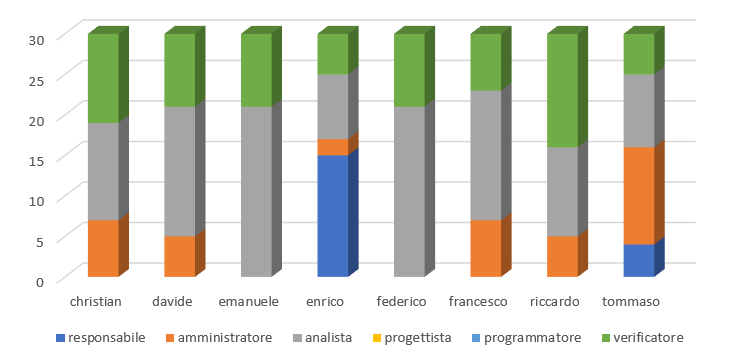
\includegraphics[scale=2.60]{Sezioni/Istogrammi/IstogrammaAnalisi.png}
	\caption{Disposizione ore per ruolo di ciascun componente della fase di Analisi}
\end{figure}

\clearpage

\subsubsection{Costo Risultante}
La seguente tabella rappresenta per ogni ruolo le ore totali investite e il corrispondente costo in euro:
{
\rowcolors{2}{grigetto}{white}
\renewcommand{\arraystretch}{2}
\begin{longtable}{ C{3cm} C{2cm} C{4cm}}
\caption{Tabella del costo risultante di Analisi}\\
\rowcolor{darkblue}

\textcolor{white}{\textbf{Ruolo}} & 
\textcolor{white}{\textbf{Totale ore}} & 
\textcolor{white}{\textbf{Costo ruolo in euro}}\\	
\endhead

Responsabile    &  19 &  570 \\
Amministratore  &  38 &  760 \\
Analista        & 114 & 2850 \\
Progettista     &   0 &    0 \\
Programmatore   &   0 &    0 \\
Verificatore    &  69 & 1035 \\
\textbf{Totale} & 240 & 5215 \\
		
\end{longtable}
}

La quantità di ore totali per ciascun ruolo viene rappresentata nel seguente areogramma:
\begin{figure}[h!]
	\centering	
	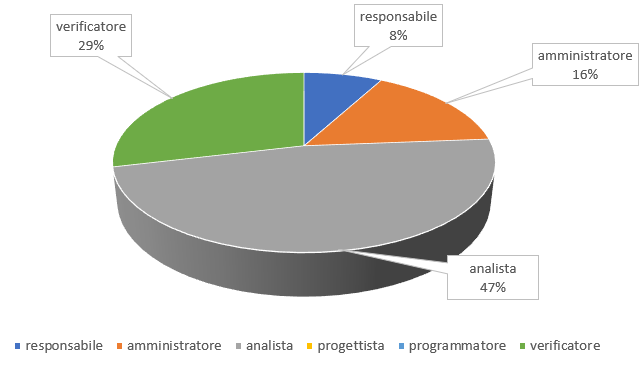
\includegraphics[scale=3.0]{Sezioni/Aerogrammi/AerogrammaAnalisi.png}
	\caption{Suddivisione ore per ruolo della fase di Analisi}
\end{figure}


\clearpage
\subsection{Progettazione Architetturale}

\subsubsection{Divisione Oraria}
La seguente tabella rappresenta la distribuzione oraria dei ruoli per ogni componente del gruppo:
{
\rowcolors{2}{grigetto}{white}
\renewcommand{\arraystretch}{2}
\begin{longtable}[h!] { C{4cm} C{1cm} C{1cm} C{1cm} C{1cm} C{1cm} C{1cm} C{3cm}}
\caption{Tabella della divisione oraria della Progettazione Architetturale}\\
\rowcolor{darkblue}

\textcolor{white}{\textbf{Membro del gruppo}} & 
\textcolor{white}{\textbf{RE}} & 
\textcolor{white}{\textbf{AM}} & 
\textcolor{white}{\textbf{AN}} & 
\textcolor{white}{\textbf{PT}} & 
\textcolor{white}{\textbf{PR}} & 
\textcolor{white}{\textbf{VE}} & 
\textcolor{white}{\textbf{Ore complessive}}\\	
\endhead
        
\MC{}                     &  5 &  - &  - & 14 & 10 &  4 &  33 \\
\LD{}                     &  8 &  - &  - & 18 &  - &  7 &  33 \\
\CE{}                     &  - &  8 &  - & 10 &  5 &  6 &  29 \\
\SE{}                     &  - & 10 &  6 & 10 &  - &  6 &  32 \\
\PF{}                     &  - &  6 &  - &  5 &  7 & 13 &  31 \\
\DF{}                     &  - &  - & 13 &  5 &  7 &  6 &  31 \\
\BR{}                     &  6 &  - &  - &  - & 17 &  8 &  31 \\
\AT{}                     &  - &  - &  8 &  7 &  - & 16 &  31 \\
\textbf{Ore totali ruolo} & 19 & 24 & 27 & 69 & 46 & 66 & 251 \\
		
\end{longtable}
}

La suddivisione delle ore svolte da ciascun componente del gruppo per ogni ruolo viene rappresentata nel seguente istogramma:
\begin{figure}[h!]
	\centering
	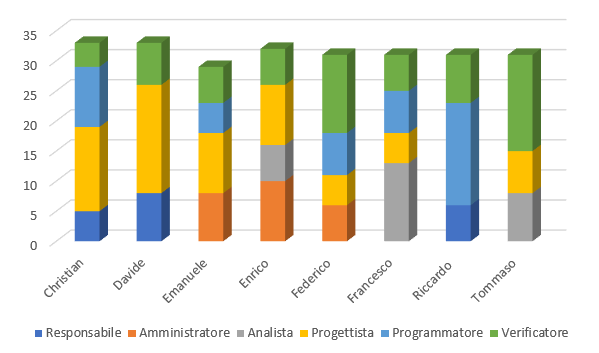
\includegraphics{Sezioni/Istogrammi/IstogrammaProgettArchitetturale.png}
	\caption{Disposizione ore per ruolo di ciascun componente della fase di Progettazione Architetturale}
\end{figure}

\clearpage

\subsubsection{Costo Risultante}
La seguente tabella rappresenta per ogni ruolo le ore totali investite e il corrispondente costo in euro:
{
\rowcolors{2}{grigetto}{white}
\renewcommand{\arraystretch}{2}
\begin{longtable}{ C{3cm} C{2cm} C{4cm}}
\caption{Tabella del costo risultante della Progettazione Architetturale}\\
\rowcolor{darkblue}

\textcolor{white}{\textbf{Ruolo}} & 
\textcolor{white}{\textbf{Totale ore}} & 
\textcolor{white}{\textbf{Costo ruolo (in \euro{})}}\\	
\endhead
        
Responsabile    &  19 &  570 \\
Amministratore  &  24 &  480 \\
Analista        &  27 &  675 \\
Progettista     &  69 & 1518 \\
Programmatore   &  46 &  690 \\
Verificatore    &  66 &  990 \\
\textbf{Totale} & 251 & 4923 \\	
        	
\end{longtable}
}

LaLa quantità di ore totali per ciascun ruolo viene rappresentata nel seguente areogramma:
\begin{figure}[h!]
	\centering
	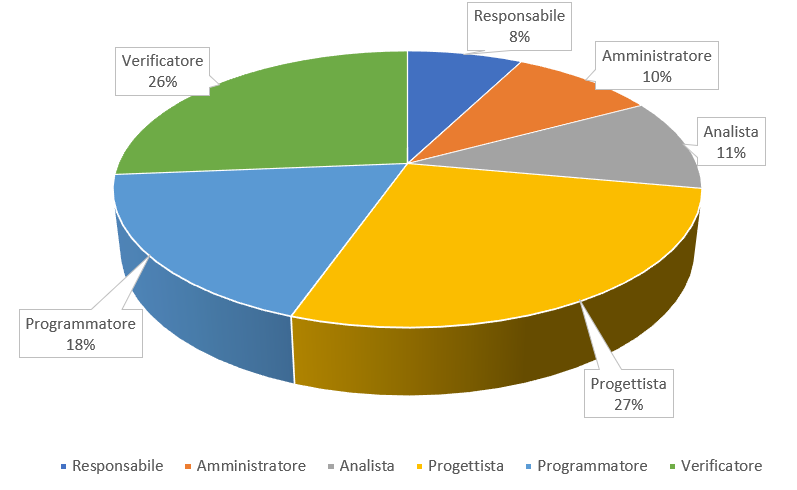
\includegraphics{Sezioni/Aerogrammi/AerogrammaProgettArchitetturale.png}
	\caption{Suddivisione ore per ruolo della fase di Progettazione Architetturale}
\end{figure}

\clearpage
\subsection{Progettazione di dettaglio e codifica}

\subsubsection{Divisione Oraria}
La seguente tabella rappresenta la distribuzione oraria dei ruoli per ogni componente del gruppo:
{
\rowcolors{2}{grigetto}{white}
\renewcommand{\arraystretch}{2}
\begin{longtable}[h!] { C{4cm} C{1cm} C{1cm} C{1cm} C{1cm} C{1cm} C{1cm} C{3cm}}
\caption{Tabella della divisione oraria della Progettazione di Dettaglio e Codifica}\\
\rowcolor{darkblue}

\textcolor{white}{\textbf{Membro del gruppo}} & 
\textcolor{white}{\textbf{RE}} & 
\textcolor{white}{\textbf{AM}} & 
\textcolor{white}{\textbf{AN}} & 
\textcolor{white}{\textbf{PT}} & 
\textcolor{white}{\textbf{PR}} & 
\textcolor{white}{\textbf{VE}} & 
\textcolor{white}{\textbf{Ore complessive}}\\
\endhead

\MC{}                     &  - & 10 & - & 13 &  16 &  11 &  50 \\
\LD{}                     &  6 &  - & - & 11 &  16 &  17 &  50 \\
\CE{}                     &  - &  5 & - & 14 &  17 &  14 &  50 \\
\SE{}                     &  - &  4 & - & 12 &  19 &  15 &  50 \\
\PF{}                     &  - &  8 & - &  9 &  20 &  13 &  50 \\
\DF{}                     & 10 &  - & - &  8 &  18 &  14 &  50 \\
\BR{}                     &  - &  3 & - & 13 &  20 &  14 &  50 \\
\AT{}                     & 10 &  - & - & 11 &  18 &  11 &  50 \\
\textbf{Ore totali ruolo} & 26 & 30 & - & 91 & 144 & 109 & 400 \\

\end{longtable}
}

La suddivisione di quante ore, ciascun componente del gruppo, ha svolto per ogni ruolo viene rappresentata nel seguente istogramma:
\begin{figure}[h!]
\centering
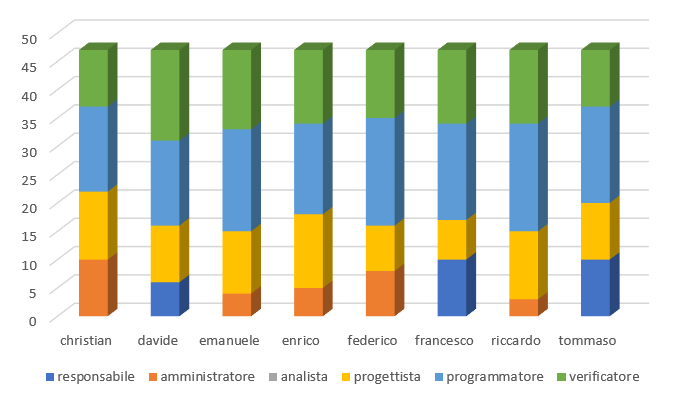
\includegraphics{Sezioni/Istogrammi/IstogrammaDiDettaglio.png}
\caption{Disposizione ore per ruolo di ciascun componente della fase di Progettazione di Dettaglio e Codifica}
\end{figure}

\clearpage

\subsubsection{Costo Risultante}
La seguente tabella rappresenta, per ruolo, le ore totali investite e il corrispondente costo in euro:
{
\rowcolors{2}{grigetto}{white}
\renewcommand{\arraystretch}{2}
\begin{longtable}{ C{3cm} C{2cm} C{4cm}}
\caption{Tabella del costo risultante della Programmazione di Dettaglio e Codifica}\\
\rowcolor{darkblue}

\textcolor{white}{\textbf{Ruolo}} & 
\textcolor{white}{\textbf{Totale ore}} & 
\textcolor{white}{\textbf{Costo ruolo (in \euro{})}}\\	
\endhead
        
Responsabile    &  26 &  780 \\
Amministratore  &  30 &  600 \\
Analista        &   - &    - \\
Progettista     &  91 & 2002 \\
Programmatore   & 144 & 2160 \\
Verificatore    & 109 & 1635 \\
\textbf{Totale} & 400 & 7177 \\
		
\end{longtable}
}

La quantità di ore totali per ciascun ruolo viene rappresentata nel seguente areogramma:
\begin{figure}[h!]
	\centering	
	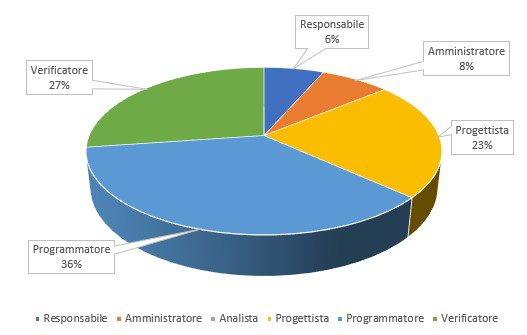
\includegraphics{Sezioni/Aerogrammi/AerogrammaDiDettaglio.png}
	\caption{Suddivisione ore per ruolo della fase di Progettazione di Dettaglio e Codifica}
\end{figure}

\clearpage
\subsection{Validazione e Collaudo}

\subsubsection{Divisione oraria}
La seguente tabella rappresenta la distribuzione oraria dei ruoli per ogni componente del gruppo:
{
\rowcolors{2}{grigetto}{white}
\renewcommand{\arraystretch}{2}
\begin{longtable}[h!] { C{4cm} C{1cm} C{1cm} C{1cm} C{1cm} C{1cm} C{1cm} C{3cm}}
\caption{Tabella della divisione oraria di Validazione e Collaudo}\\
\rowcolor{darkblue}

\textcolor{white}{\textbf{Membro del gruppo}} & 
\textcolor{white}{\textbf{RE}} & 
\textcolor{white}{\textbf{AM}} & 
\textcolor{white}{\textbf{AN}} & 
\textcolor{white}{\textbf{PT}} & 
\textcolor{white}{\textbf{PR}} &
\textcolor{white}{\textbf{VE}} &
\textcolor{white}{\textbf{Ore complessive}}\\	
\endhead
        
\MC{}                     &  - &  - &  7 &  - &  4 &  8 &  19 \\
\LD{}                     &  - &  4 &  - &  5 &  - & 10 &  19 \\
\CE{}                     &  5 &  - &  - &  - &  6 & 12 &  23 \\ 
\SE{}                     &  - &  - &  - &  6 &  5 &  9 &  20 \\
\PF{}                     &  6 &  - &  - &  - &  7 &  8 &  21 \\
\DF{}                     &  - &  6 &  - &  - &  9 &  6 &  21 \\
\BR{}                     &  - &  5 &  - &  - &  6 & 10 &  21 \\
\AT{}                     &  - &  - &  4 & 10 &  - &  7 &  21 \\
\textbf{Ore totali ruolo} & 11 & 15 & 11 & 21 & 37 & 70 & 165 \\
		
\end{longtable}
}


La suddivisione delle ore svolte da ciascun componente del gruppo per ogni ruolo viene rappresentata nel seguente istogramma:
\begin{center}
	\pgfplotsset{width=17cm, height=8.5cm}
	\begin{tikzpicture}
		\begin{axis}[
			ybar stacked,
			bar width=20pt,
			legend style={
				at={(0.5,-0.15)},
				anchor=north,
				legend columns=-1
			},
			symbolic x coords={Christian, Davide, Emanuele, Enrico, Federico, Francesco, Riccardo, Tommaso},
			xtick=data
		]
			\legend{Responsabile, Amministratore, Analista, Progettista, Programmatore, Verificatore}
			% Responsabile
			\addplot [ybar, fill=blue] coordinates {\ColonnaIstogramma{0}{0}{5}{0}{6}{0}{0}{0}};
			% Amministratore
			\addplot [ybar, fill=yellow] coordinates {\ColonnaIstogramma{0}{4}{0}{0}{0}{6}{5}{0}};
			% Analista
			\addplot [ybar, fill=red] coordinates {\ColonnaIstogramma{7}{0}{0}{0}{0}{0}{0}{4}};
			% Progettista
			\addplot [ybar, fill=green] coordinates {\ColonnaIstogramma{0}{5}{0}{6}{0}{0}{0}{10}};
			% Programmatore
			\addplot [ybar, fill=grigetto] coordinates {\ColonnaIstogramma{4}{0}{6}{5}{7}{9}{6}{0}};
			% Verificatore
			\addplot [ybar, fill=orange] coordinates {\ColonnaIstogramma{8}{10}{12}{9}{8}{6}{10}{7}};
		\end{axis}
	\end{tikzpicture}
\end{center}
\clearpage

\clearpage

\subsubsection{Costo risultante}
La seguente tabella rappresenta rappresenta per ogni ruolo le ore totali investite e il corrispondente costo in euro:
{
\rowcolors{2}{grigetto}{white}
\renewcommand{\arraystretch}{2}
\begin{longtable}{ C{3cm} C{2cm} C{4cm}}
\caption{Tabella del costo risultante di Validazione e Collaudo}\\
\rowcolor{darkblue}

\textcolor{white}{\textbf{Ruolo}} & 
\textcolor{white}{\textbf{Totale ore}} & 
\textcolor{white}{\textbf{Costo ruolo (in \euro{})}}\\	
\endhead
        
Responsabile    &  11 &  330 \\
Amministratore  &  15 &  300 \\
Analista        &  11 &  275 \\
Progettista     &  21 &  462 \\
Programmatore   &  37 &  555 \\
Verificatore    &  70 & 1050 \\
\textbf{Totale} & 169 & 2972 \\
	
\end{longtable}
}

\vskip 100pt %spazio verticale
La quantità di ore totali per ciascun ruolo viene rappresentata nel seguente areogramma:
\begin{center}
	\begin{tikzpicture}
		\pie[rotate = 180, color={blue, yellow, red, green, grigetto, orange}] {
			7/Responsabile,
			9/Amministratore,
			7/Analista,
			13/Progettista,
			22/Programmatore,
			42/Verificatore
		}
	\end{tikzpicture}
\end{center}


\clearpage
\subsection{Preventivo finale} 
Nel preventivo riportiamo la spesa totale che il committente dovrà affrontare, derivata dal totale delle ore rendicontate e preventivate nelle fasi di Progettazione Architetturale, Progettazione di Dettaglio e Codifica, Validazione e Collaudo.

\subsubsection{Divisione oraria complessiva} 
La seguente tabella rappresenta la distribuzione oraria dei ruoli per ogni componente del gruppo:
{
\rowcolors{2}{grigetto}{white}
\renewcommand{\arraystretch}{2}
\begin{longtable}[h!] { C{4cm} C{1cm} C{1cm} C{1cm} C{1cm} C{1cm} C{1cm} C{3cm}}
\caption{Tabella della divisione oraria complessiva}\\
\rowcolor{darkblue}

\textcolor{white}{\textbf{Membro del gruppo}} & 
\textcolor{white}{\textbf{RE}} & 
\textcolor{white}{\textbf{AM}} & 
\textcolor{white}{\textbf{AN}} & 
\textcolor{white}{\textbf{PT}} & 
\textcolor{white}{\textbf{PR}} & 
\textcolor{white}{\textbf{VE}} & 
\textcolor{white}{\textbf{Ore complessive}}\\	
\endhead
        
\MC{}                     &  5 & 10 &  7 &  27 &  30 &  23 & 102 \\
\LD{}                     & 14 &  4 &  - &  34 &  16 &  34 & 102 \\
\CE{}                     &  5 & 13 &  - &  24 &  28 &  32 & 102 \\
\SE{}                     &  - & 14 &  6 &  28 &  24 &  30 & 102 \\
\PF{}                     &  6 & 14 &  - &  14 &  34 &  34 & 102 \\
\DF{}                     & 10 &  6 & 13 &  13 &  34 &  26 & 102 \\
\BR{}                     &  6 &  8 &  - &  13 &  43 &  32 & 102 \\
\AT{}                     & 10 &  - & 12 &  28 &  18 &  34 & 102 \\
\textbf{Ore totali ruolo} & 56 & 69 & 38 & 181 & 227 & 245 & 816 \\

\end{longtable}
}

\subsubsection{Costo complessivo per ruolo}
Nella seguente tabella viene illustrato il monte ore risultante per ogni ruolo con il costo ad esso associato:
{
\rowcolors{2}{grigetto}{white}
\renewcommand{\arraystretch}{2}
\begin{longtable}{ C{3cm} C{2cm} C{4cm}}
\caption{Tabella del costo complessivo per ruolo}\\
\rowcolor{darkblue}

\textcolor{white}{\textbf{Ruolo}} & 
\textcolor{white}{\textbf{Totale ore}} & 
\textcolor{white}{\textbf{Costo ruolo (in \euro{})}}\\	
\endhead
        
Responsabile   &  56 & 1680 \\
Amministratore &  69 & 1380 \\
Analista       &  38 &  950 \\
Progettista    & 181 & 3982 \\
Programmatore  & 227 & 3405 \\
Verificatore   & 245 & 3675 \\
        	
\end{longtable}
}

\subsubsection{Costo complessivo}
Nella seguente tabella vengono riportati i costi complessivi delle varie fasi e infine l'importo proposto da \Gruppo{} per la realizzazione del progetto \NomeProgetto{}:\\
{
\rowcolors{2}{grigetto}{white}
\renewcommand{\arraystretch}{2}
\begin{longtable}{ C{5cm} C{5cm}}
\caption{Tabella del costo complessivo}\\
\rowcolor{darkblue}

\textcolor{white}{\textbf{Fase}} &
\textcolor{white}{\textbf{Costo Fase}}\\	
\endhead
		
Progettazione Architetturale          &  4923 \\
Progettazione di Dettaglio e Codifica &  7177 \\
Validazione e Collaudo                &  2972 \\
\textbf{Totale}                       & 15072 \\

\end{longtable}
}